\documentclass[a4paper, 12pt]{article}
\usepackage[utf8]{inputenc}
\usepackage[T1]{fontenc}
\usepackage[polish]{babel}
\usepackage{graphicx}
\usepackage{hyperref}
\usepackage{listings}
\usepackage{xcolor}

\title{Dokumentacja aplikacji Unordered}
\author{Adam Dybcio\endline Łukasz Czapski\endline Igor Ciżewski\endline Denis Jabłoński\endline Mateusz Sztankiewicz}
\date{\today}

\begin{document}

\maketitle
\newpage
\tableofcontents
\newpage

\section{Wprowadzenie}
\subsection{Cel dokumentu}
opisać cel dokumentu

\subsection{Opis aplikacji}
opisać krótko aplikacje i jej funkcjonalności
\begin{itemize}
    \item Tworzenie "boxów prezentów" (zestawów propozycji),
    \item Konfigurowanie cyklicznych generowań (np. co roku na urodziny),
    \item Losowanie całkowicie przypadkowych propozycji.
\end{itemize}

\newpage
\section{Architektura}
\subsection{Diagram wysokopoziomowy}
\begin{figure}[ht]
    \centering
    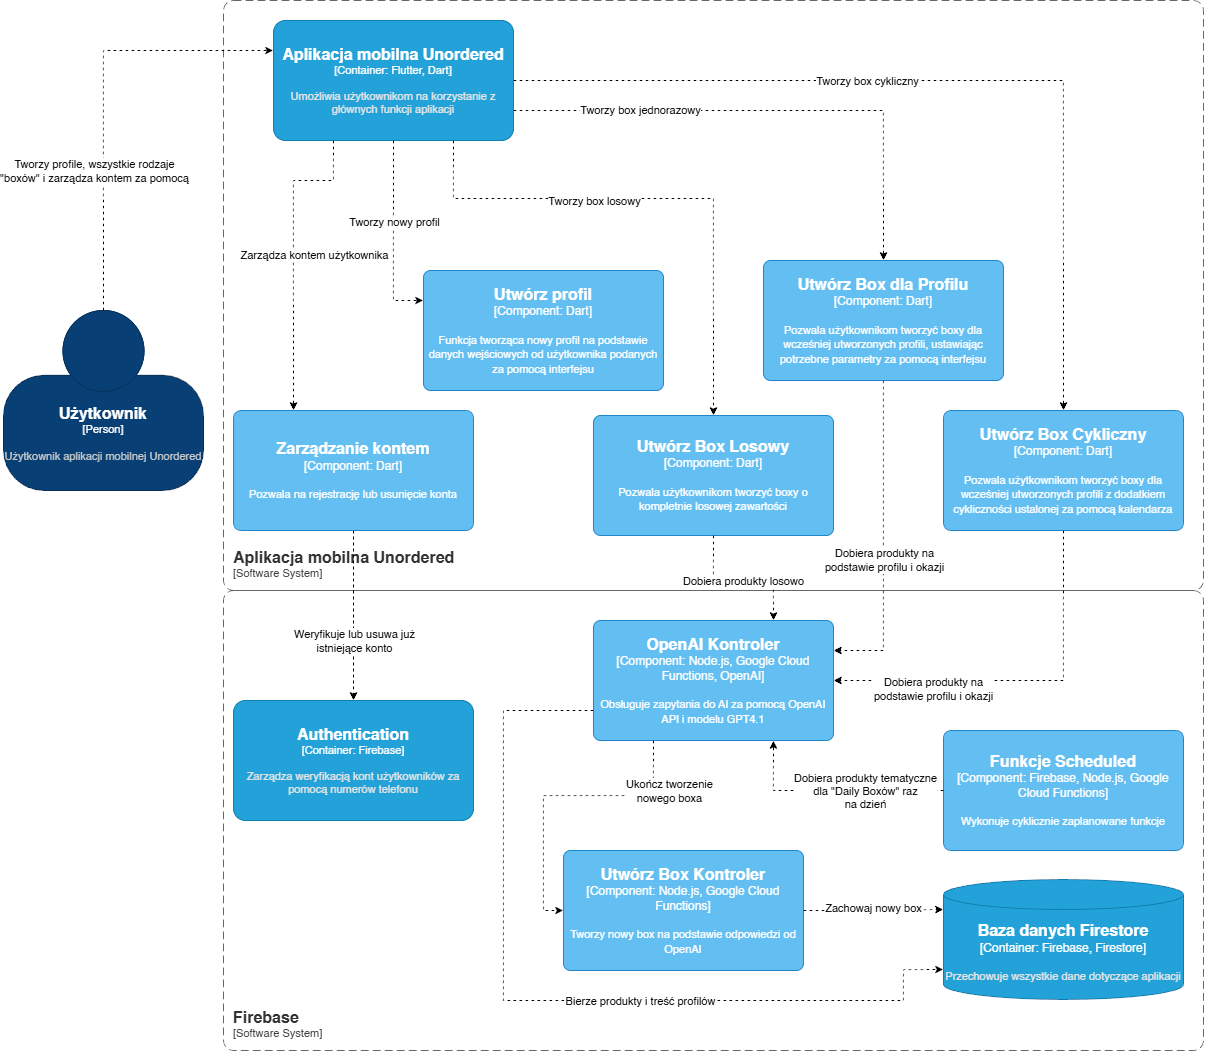
\includegraphics[width=1\textwidth]{images/unordered.c4.png}
    \caption{Architektura systemu}{Źródło: drawio.com}
    \label{fig:arch}
\end{figure}

\subsection{Frontend (Flutter)}
\begin{itemize}
    \item Wersja Flutter: [X.Y.Z]
    \item Główne pakiety: \texttt{firebase\_core}, \texttt{cloud\_functions}, \texttt{http}, etc.
    \item Struktura katalogów:
    \begin{lstlisting}[language=bash]
    \end{lstlisting}
\end{itemize}

\subsection{Backend (Firebase)}
\begin{itemize}
    \item Cloud Functions (Node.js)
    \item Firestore (baza danych)
    \item Authentication (logowanie)
    \item Integracja z OpenAI API
\end{itemize}

\newpage
\section{Funkcjonalności}
\subsection{Generowanie prezentów}
\subsubsection{Profil użytkownika}
Opis pól profilu (np. wiek, zainteresowania, budżet).

\subsubsection{Typy generowania}
\begin{itemize}
    \item \textbf{Na teraz} – jednorazowe generowanie dla podanych parametrów
    \item \textbf{Cykliczne} – konfiguracja powtarzalnych generowań
    \item \textbf{Losowe} – bez podawania parametrów
\end{itemize}

\subsection{Boxy prezentów}
\begin{itemize}
    \item Struktura boxa (nazwa, data, lista propozycji)
    \item Zapisywanie historii
    \item Udostępnianie
\end{itemize}

\newpage
\section{Integracja z OpenAI}
\subsection{Prompt engineering}
Opisać prompty, które są używane do generowania prezentów.
\begin{lstlisting}[language=python]
"prompt"
\end{lstlisting}

\subsection{Przetwarzanie odpowiedzi}
Opis parsowania odpowiedzi API i mapowania na model danych aplikacji.

\newpage
\section{Wdrożenie}
\subsection{Konfiguracja Firebase}
Instrukcja deploy funkcji cloudowych:
\begin{lstlisting}[language=bash]
firebase deploy --only functions
\end{lstlisting}

\subsection{Środowiska}
\begin{itemize}
    \item Development
    \item Production
\end{itemize}

\newpage
\section{Testowanie}
\subsection{Testy jednostkowe}
\begin{itemize}
    \item Flutter (widget tests)
    \item Cloud Functions (Jest/Mocha)
\end{itemize}

\subsection{Testy integracyjne}
Scenariusze testowe dla głównych ścieżek.

\newpage
\section{Podsumowanie i dalszy rozwój}
\subsection{Znane ograniczenia}
\begin{itemize}
    \item Ograniczenia OpenAI (np. długość promptów)
    \item Limity Firebase
\end{itemize}

\subsection{Roadmap}
Planowane funkcje (np. integracja z sklepami online).

\begin{thebibliography}{9}
\bibitem{flutter}
Flutter documentation, \url{https://flutter.dev/docs}

\bibitem{firebase}
Firebase documentation, \url{https://firebase.google.com/docs}

\bibitem{openai}
OpenAI API reference, \url{https://platform.openai.com/docs/api-reference}
\end{thebibliography}

\end{document}